\documentclass[aspectratio=169,11pt]{beamer}
\makeatletter
\input{../../templates/dune-professional/beamerthemeDUNEProfessional.sty}
\makeatother
\title{VD detector protection}
\subtitle{System interfaces, proposed interlocks and hardware additions}
\author{Manuel Arroyave}
\date{I\&I workshop --- 28 October 2026}
\newcommand{\mydate}{28 October 2026}
\hypersetup{colorlinks=true,urlcolor=DuneInfo,linkcolor=DuneInfo}
\newcommand{\captionline}[1]{\par{\small\color{DuneTextMuted}#1\par}}
% Schematic service boundary, not a surveyed section or controller inventory.
\newcommand{\siteboundarymap}[2]{%
\begin{tikzpicture}[
 box/.style={text=DuneOnAccent,align=center,font=\small,inner sep=4pt},
 level/.style={anchor=east,font=\small,text=DuneTextMuted}]
 \node[font=\small\bfseries,align=center,text width=2.0cm] at (1.25,2.25) {SDSTA\\site services};
 \node[font=\small\bfseries,align=center,text width=2.8cm] at (4.05,2.25) {FFDG DUNE FD\\building services};
 \draw[draw=DuneBorder,line width=1pt] (0.05,1.83) -- (5.6,1.83);
 \draw[draw=DuneSky,line width=2pt] (1.25,1.55) -- (1.25,-1.85);
 \node[level] at (-0.05,1.25) {Surface};
 \node[box,fill=#1,text width=1.95cm] at (1.25,1.25) {Oro Hondo\\Ross shaft};
 \node[level] at (-0.05,0.25) {4850};
 \draw[draw=DuneBorder] (0.05,0.25) -- (5.6,0.25);
 \node[box,fill=#2,text width=2.8cm] at (4.05,0.25) {CUC / caverns\\HVAC, chilled water};
 \node[level] at (-0.05,-0.85) {4910};
 \draw[draw=DuneBorder] (0.05,-0.85) -- (5.6,-0.85);
 \node[box,fill=#2,text width=2.8cm] at (4.05,-0.85) {SP-1 / SP-2\\sump interfaces};
 \node[box,fill=#1,text width=1.95cm] at (1.25,-1.85) {Mine drainage\\and pumping};
 \draw[-{Stealth},draw=DuneSky,line width=1pt] (3.1,-1.3) -- (2.35,-1.65);
\end{tikzpicture}%
}

\hyphenpenalty=10000
\exhyphenpenalty=10000
\begin{document}
\begin{frame}{Definitions and responsibilities}
\renewcommand{\arraystretch}{1.18}
\begin{tabularx}{\textwidth}{@{}>{\RaggedRight\arraybackslash}p{2.2cm}>{\RaggedRight\arraybackslash}X@{}}
\textbf{DPS} & Detector Protection System: arbitrates protection, applies permits and inhibits, and checks the response.\\
\textbf{SC} & Slow controls: operates and monitors equipment, coordinates requests and keeps the logs.\\
\textbf{DAQ} & Data acquisition: configures readout and records detector data.\\
\textbf{BMS / cryo} & Building management and cryogenics: operate their systems and report their state to SC.\\
\textbf{Subsystems} & Define operating limits, protection actions and allowed response times.\\
\textbf{Local\newline interlocks} & Can trip equipment without SC or the central DPS.\\
\end{tabularx}\par\bigskip
\textbf{Protection trips take priority over operating requests.}\par\medskip
SDSTA issues personnel-safety alarms.
\end{frame}

\begin{frame}{How the systems connect}
\centering
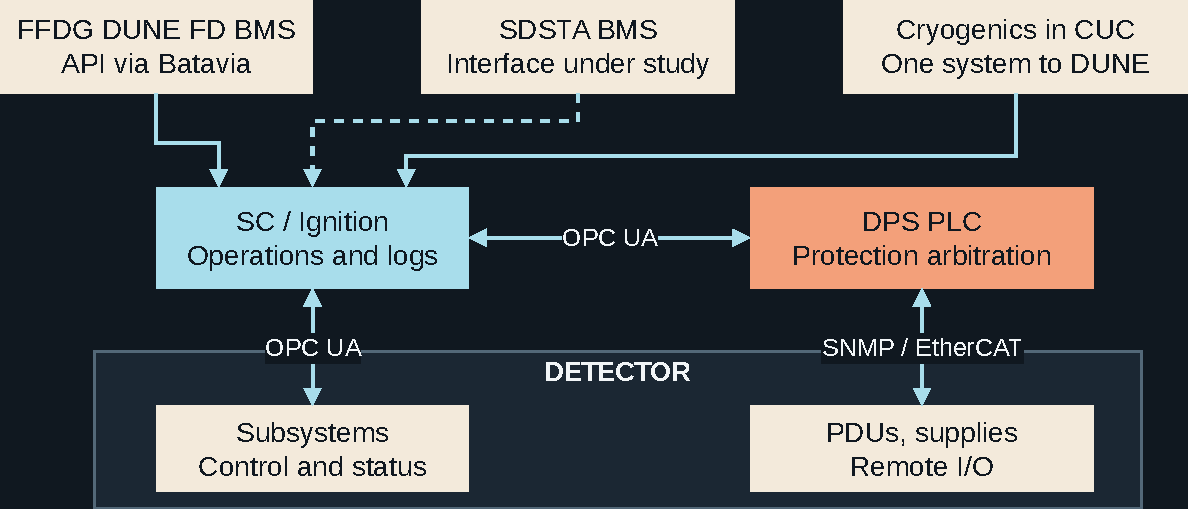
\includegraphics[width=\textwidth,height=4.6cm,keepaspectratio]{figures/drawio-overview.pdf}\par\bigskip
\raggedright

OPC UA carries status and requests. DPS uses SNMP for power distribution units (PDUs) and supplies, and EtherCAT for remote I/O.
\end{frame}

\begin{frame}{FFDG BMS: the building-services interface}
\begin{columns}[T,onlytextwidth]
\begin{column}{0.51\textwidth}
\centering\siteboundarymap{DunePaper}{DuneSky}
\end{column}
\begin{column}{0.47\textwidth}
\textbf{Proposed connection}\par
ISD proposes a Metasys API in Batavia to connect the FFDG DUNE FD BMS to SC.\par\bigskip
\textbf{Tested with SBN building data}\par
The API and OPC UA publication have been exercised.\par\bigskip
\textbf{Needed for live data}\par
The Metasys API licence.
\end{column}
\end{columns}\par\bigskip
\captionline{Service boundaries at SURF. The map shows the scope of the systems, not individual controllers.}
\end{frame}

\begin{frame}{SDSTA BMS: survey and interface status}
\begin{columns}[T,onlytextwidth]
\begin{column}{0.51\textwidth}
\centering\siteboundarymap{DuneCoral}{DunePaper}
\end{column}
\begin{column}{0.47\textwidth}
\textbf{Hardware survey underway}\par
Locate controllers, input/output connections and network ports.\par\bigskip
\textbf{Protocols under investigation}\par
Find which signals can be sent to SC.\par\bigskip
\textbf{Agreement under discussion}\par
Set responsibilities for signal use, faults and maintenance.
\end{column}
\end{columns}\par\bigskip
\captionline{SDSTA services extend beyond the detector caverns. The survey will establish the BMS connection points.}
\end{frame}

\begin{frame}{Cryogenics: one system to DUNE}
The cryogenic controls are in the Central Utility Cavern (CUC).
Their internal divisions appear as one system to DUNE.\par\bigskip
\renewcommand{\arraystretch}{1.3}
\begin{tabularx}{\textwidth}{@{}>{\RaggedRight\arraybackslash}p{3cm}>{\RaggedRight\arraybackslash}X@{}}
\toprule
\textbf{Function} & \textbf{Detector interface}\\\midrule
Process control & Cryogenics operates and protects its own process.\\
Protection inputs & Liquid-argon level, relief-valve state and boiling-risk conditions can affect HV and bias permits.\\
Information path & Cryogenics $\rightarrow$ SC $\leftrightarrow$ DPS. Trace each measurement to its actual sensor.\\
Before operation & Agree readiness states, limits and the response to missing or invalid data.\\
\bottomrule
\end{tabularx}\par\medskip
The detector running conditions are still being agreed.
\end{frame}

\begin{frame}{Use the interlock matrix to review each system}
\centering
\begin{tikzpicture}[
 box/.style={fill=DunePaper,text=DuneOnAccent,align=center,text width=2.2cm,minimum height=1.25cm,inner sep=5pt,font=\small},
 edge/.style={-{Stealth},draw=DuneSky,line width=1.2pt}]
 \node[box] (s) at (-5.5,0) {Condition\\and source};
 \node[box] (i) at (-2.75,0) {Physical input\\and connection};
 \node[box,fill=DuneSky] (c) at (0,0) {DPS / local\\decision};
 \node[box,fill=DuneCoral] (o) at (2.75,0) {Action and\\equipment};
 \node[box] (f) at (5.5,0) {Equipment state\\and feedback};
 \draw[edge] (s)--(i);\draw[edge] (i)--(c);\draw[edge] (c)--(o);\draw[edge] (o)--(f);
 \end{tikzpicture}\par\bigskip
\raggedright

Start with the interlocks proposed by the consortia in their interface documents (ICDs).\par\bigskip
For each one, identify the existing hardware, missing connections and required additions. Check the time from detection to completed shutdown.\par\bigskip
\textbf{Use the rack lists, drawings, parts lists and power calculations.}
\end{frame}

\begin{frame}{DPS logic: allow, trip and recover}
\centering
\begin{tikzpicture}[
 box/.style={fill=DunePaper,text=DuneOnAccent,align=center,text width=2.65cm,minimum height=1.4cm,inner sep=5pt,font=\small},
 edge/.style={-{Stealth},draw=DuneSky,line width=1.2pt}]
 \node[box] (i) at (-5.1,0) {Conditions\\and SC requests};
 \node[box,fill=DuneSky] (l) at (-1.7,0) {DPS PLC\\protection rules};
 \node[box,fill=DuneCoral] (a) at (1.7,0) {Permits / inhibits\\SNMP or wired I/O};
 \node[box] (f) at (5.1,0) {Equipment state\\and feedback};
 \draw[edge] (i)--(l);\draw[edge] (l)--(a);\draw[edge] (a)--(f);
 \end{tikzpicture}\par\bigskip
\raggedright

\textbf{Allow:} the request is valid, required conditions are met and no trip is active.\par\medskip
\textbf{Trip:} remove the permit, retain the cause and check the equipment response. SC logs the event.\par\medskip
\textbf{Recover:} reset the trip, then request a separate re-enable.\par\bigskip
\captionline{Proposed controller: a commercial programmable logic controller (PLC) based on BDE, located in the CUC. Loss-of-signal behaviour is set for each protected load.}
\end{frame}

\begin{frame}{Detector}

\end{frame}

\begin{frame}{BDE: the existing bottom-drift design}
\centering
\begin{tikzpicture}[
 box/.style={fill=DunePaper,text=DuneOnAccent,align=center,text width=3.1cm,minimum height=1.05cm,inner sep=6pt},
 edge/.style={-{Stealth},draw=DuneSky,line width=1.2pt}]
 \node[box,fill=DuneSky] (io) at (-4,0) {Auxiliary rack\\remote I/O};
 \node[box] (lv) at (1.6,1.1) {2 LV racks\\2 PL506 supplies};
 \node[box,fill=DuneCoral] (wiec) at (1.6,-1.1) {8 warm crates\\8 PTCs + 48 WIBs};
 \draw[edge] (io.north east) -| (-1.7,1.1) -- node[above,font=\small] {inhibits} (lv.west);
 \draw[arrows={Stealth-Stealth},draw=DuneSky,line width=1.2pt] (io.south east) -| (-1.7,-1.1) -- node[below,font=\small] {EtherCAT} (wiec.west);
 \draw[edge] (lv.east) -- (4.35,1.1) -- node[right,font=\small] {48 V} (4.35,-1.1) -- (wiec.east);
 \end{tikzpicture}\par\bigskip
\raggedright

\textbf{Ten groups:} 10 auxiliary racks, 20 low-voltage racks and 20 PL506 supplies; 80 warm interface electronics crates (WIECs), containing 480 interface boards (WIBs).\par\medskip
Each crate has a power and timing card (PTC). Ten bias racks provide the separate charge-readout-plane and field-cage interfaces.\par\medskip
\textbf{Available:} panel drawings, parts lists, power calculations and Ignition screens.
\end{frame}

\begin{frame}{BDE trip example: loss of fan cooling}
\centering
\begin{tikzpicture}[
 box/.style={fill=DunePaper,text=DuneOnAccent,align=center,text width=2.35cm,minimum height=1.05cm,inner sep=5pt,font=\small},
 edge/.style={-{Stealth},draw=DuneSky,line width=1.2pt}]
 \node[box] (fan) at (-5.1,0) {Fan-status input};
 \node[box,fill=DuneSky] (plc) at (-1.7,0) {DPS PLC\\cooling rule};
 \node[box,fill=DuneCoral] (lv) at (1.7,1) {Remote output\\PL506 inhibit};
 \node[box] (wiec) at (5.1,1) {Affected WIEC\\48 V off};
 \node[box,fill=DuneCoral] (bias) at (1.7,-1) {Remote output\\ISEG inhibit};
 \node[box] (crp) at (5.1,-1) {Associated\\bias off};
 \draw[edge] (fan)--node[above=18pt,font=\small] {EtherCAT}(plc);
 \draw[edge] (plc.north east) |- (lv.west);\draw[edge] (lv)--(wiec);
 \draw[edge,dashed] (plc.south east) |- (bias.west);\draw[edge,dashed] (bias)--(crp);
 \end{tikzpicture}\par\bigskip
\raggedright

A cooling fault removes power from the affected crate. DPS checks the supply state and voltage; SC records the trip.\par\bigskip
\textbf{Solid path:} documented fan-to-power-supply inhibit.\par\medskip
\textbf{Dashed path:} associated bias shutdown, if required by the VD interlock rule. The dependency and shutdown order are still being agreed.
\end{frame}

\begin{frame}{PDS DAPHNE: bias control, power and DAQ}
\centering

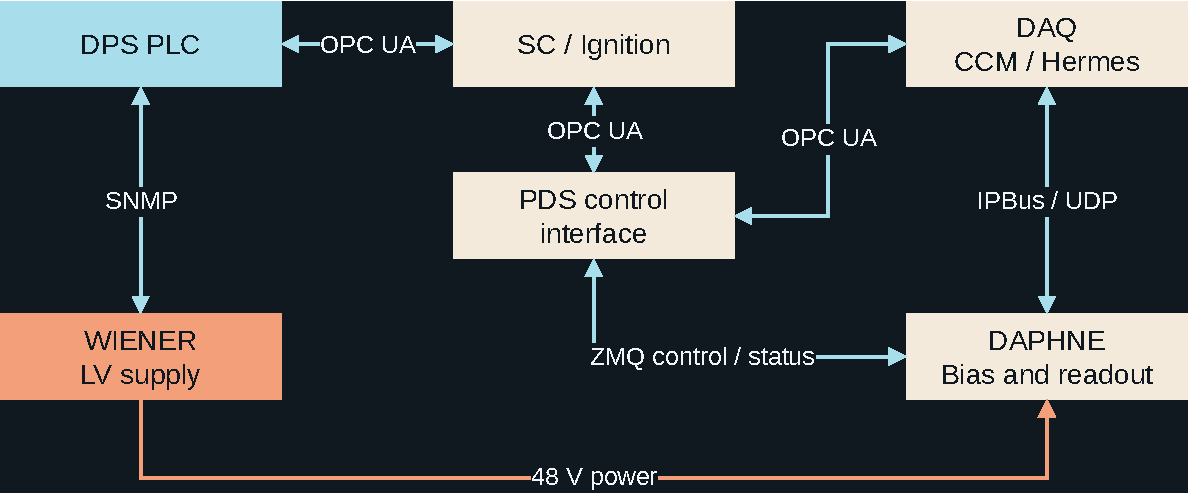
\includegraphics[width=\textwidth,height=4.6cm,keepaspectratio]{figures/drawio-daphne.pdf}
\par\bigskip
\raggedright

\textbf{Photon Detection System (PDS): 34 low-voltage feeds.}\par\medskip
SiPM light-sensor bias inhibit: DPS $\rightarrow$ SC $\rightarrow$ DAPHNE. SC returns bias status and informs DAQ. Cathode-mounted devices use the PoF path on the next slide.
\end{frame}

\begin{frame}{Power over fibre: monitor and switch off locally}
\centering

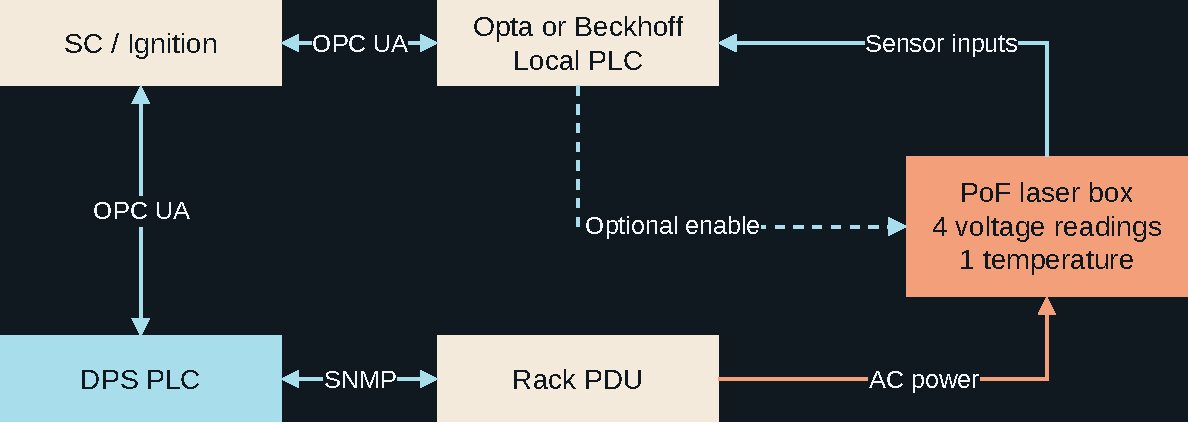
\includegraphics[width=\textwidth,height=4.6cm,keepaspectratio]{figures/drawio-pof.pdf}
\par\bigskip
\raggedright

\textbf{80 boxes: 320 voltage + 80 temperature readings = 400 readings.}\par\medskip
DPS inhibits power over fibre (PoF) through the PDU. A separate box-enable signal would provide another control option, if available.
\end{frame}

\begin{frame}{High voltage: drift and detector bias}
\textbf{One drift-HV supply; ten bias crates with 576 channels.}\par
480 channels serve the charge readout planes (CRPs); 96 serve the field cage.\par\bigskip
\renewcommand{\arraystretch}{1.35}
\begin{tabularx}{\textwidth}{@{}>{\RaggedRight\arraybackslash}p{2.1cm}>{\RaggedRight\arraybackslash}X>{\RaggedRight\arraybackslash}X@{}}
\toprule
\textbf{Equipment} & \textbf{Control and monitoring} & \textbf{Protection}\\\midrule
Heinzinger drift-HV supply & SC / OPC UA through LabVIEW and cRIO; analog control and readback & DPS remote I/O operates the wired interlock\\
ISEG bias supplies & DPS uses SNMP; SC receives status and logs & DPS remote I/O operates wired channel inhibits\\
\bottomrule
\end{tabularx}\par\bigskip
\textbf{Example:} low liquid-argon level removes the drift-HV permit. A drift-HV trip also shuts down the associated field-cage termination supplies.
\end{frame}

\begin{frame}{CalCI: temperature measurements}
\centering
\begin{tikzpicture}[
 box/.style={fill=DunePaper,text=DuneOnAccent,align=center,text width=2.5cm,minimum height=0.85cm,inner sep=5pt,font=\small},
 edge/.style={-{Stealth},draw=DuneSky,line width=1.2pt}]
 \node[box] (rtd) at (-5,1) {Temperature sensors\\RTDs};
 \node[box] (crio) at (-1.5,1) {cRIO readout\\LabVIEW};
 \node[box] (fbg) at (-5,-1) {Fibre temperature\\sensors};
 \node[box] (int) at (-1.5,-1) {Optical readout\\interrogator};
 \node[box] (sc) at (2.5,0) {SC / OPC UA\\logs and status};
 \node[box,fill=DuneSky,text width=1.5cm] (dps) at (5.8,0) {DPS};
 \draw[edge] (rtd)--(crio);\draw[edge] (fbg)--(int);
 \draw[edge] (crio.east)-| (sc.north);\draw[edge] (int.east)-| (sc.south);
 \draw[edge] (sc)--(dps);
 \end{tikzpicture}\par\bigskip
\raggedright

Calibration and Cryogenic Instrumentation (CalCI) measures conditions inside the detector. Temperature profiles guide cooldown and operation.\par\bigskip
For protection, each measurement needs a location, a limit, an allowed response time and a named piece of equipment to shut down.
\end{frame}

\begin{frame}{CalCI: ionization lasers}
\centering
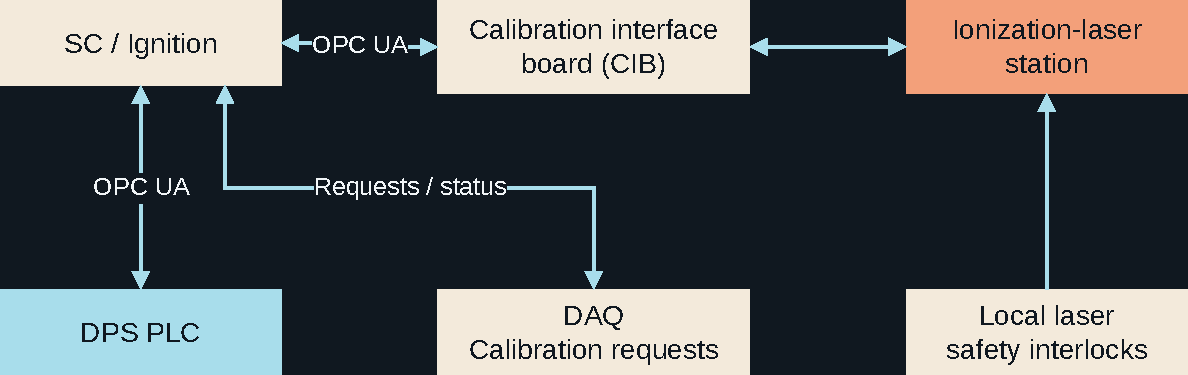
\includegraphics[width=\textwidth,height=4.6cm,keepaspectratio]{figures/drawio-lasers.pdf}\par\bigskip
\raggedright

\textbf{Four laser stations.} Proposed rule: block conflicting laser and PDS requests. Restore PDS after confirmed emission-off or shutter closure.\par\medskip
Local laser-safety interlocks remain independent.
\end{frame}

\begin{frame}{CalCI: purity monitors}
\centering
\begin{tikzpicture}[
 box/.style={fill=DunePaper,text=DuneOnAccent,align=center,text width=2.45cm,minimum height=1.2cm,inner sep=5pt,font=\small},
 edge/.style={-{Stealth},draw=DuneSky,line width=1.2pt},
 duplex/.style={arrows={Stealth[length=1.6mm,width=1.2mm]-Stealth[length=1.6mm,width=1.2mm]},draw=DuneSky,line width=1.2pt}]
 \node[box] (prm) at (-5.1,0) {Purity monitor\\Bias / lamp};
 \node[box] (read) at (-1.7,0) {Digitizer\\LabVIEW control};
 \node[box] (sc) at (1.7,0) {SC / OPC UA\\Activity and logs};
 \node[box] (daq) at (5.1,0) {DAQ\\activity tags};
 \draw[duplex] (prm)--(read);\draw[duplex] (read)--(sc);\draw[edge] (sc)--(daq);
 \end{tikzpicture}\par\bigskip
\raggedright

\textbf{Proposed approach:} keep taking data and mark the intervals when the flash lamp is active.\par\bigskip
\textbf{Decision still needed:} the older PDS interface document requires SiPM bias to be off during purity-monitor activity. Agree the rule before implementing the inhibit.
\end{frame}

\begin{frame}{Rack infrastructure: shared protection}
\centering
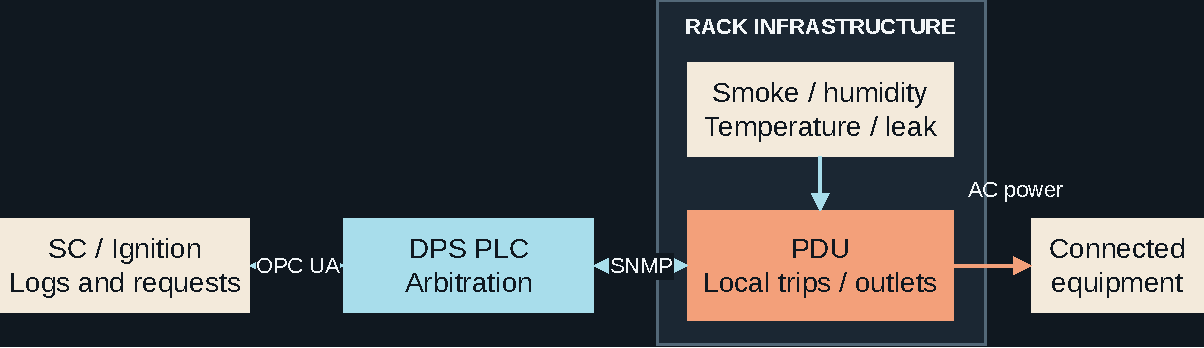
\includegraphics[width=\textwidth,height=4.6cm,keepaspectratio]{figures/drawio-racks.pdf}\par\medskip
\raggedright

Rack protection groups the PDUs, sensors and connections. Local rules switch off affected outlets. Humidity is monitored; a humidity trip needs a separate requirement.\par\medskip
\textbf{TDE + DAQ/timing: 336 microTCA crates. TDE uses 20 mezzanine racks.} DPS controls their PDUs; crate-status and external-inhibit interfaces remain possible additions.
\end{frame}

\begin{frame}{Test the complete protection path}
\centering
\begin{tikzpicture}[
    box/.style={fill=DunePaper,text=DuneOnAccent,align=center,
      text width=2.25cm,minimum height=1.0cm,inner sep=5pt},
    edge/.style={-{Stealth},draw=DuneSky,line width=1.2pt}]
    \node[box] (in) at (-4.8,0) {Fault input or\\conflicting request};
    \node[box,fill=DuneSky] (plc) at (-1.6,0) {DPS PLC\\arbitration};
    \node[box,fill=DuneCoral] (out) at (1.6,0) {Supply inhibit\\or PDU command};
    \node[box] (state) at (4.8,0) {Equipment state\\and feedback};
    \draw[edge] (in) -- (plc);
    \draw[edge] (plc) -- (out);
    \draw[edge] (out) -- (state);
  \end{tikzpicture}\par\bigskip
\raggedright

Use the existing BDE test setup to measure detection through completed shutdown.\par\medskip
Test local trips, lost communications, reset and re-enable. Check that SC logs the cause, decision and final equipment state.\par\bigskip
No critical function requiring less than 1 ms has been identified so far. The consortium review and hardware tests will check this assumption.
\end{frame}

\begin{frame}{Hardware review and procurement: June 2027}
\renewcommand{\arraystretch}{1.45}
\begin{tabularx}{\textwidth}{@{}>{\RaggedRight\arraybackslash}p{3.4cm}>{\RaggedRight\arraybackslash}X@{}}
\toprule
\textbf{Work before review} & \textbf{Result}\\\midrule
Trace each inhibit & Existing hardware, additions, cable routes and quantities\\
Test representative paths & Measured trip times, recovery and SC logging\\
Prepare purchases & Panel space, power, drawings, parts, licences, costs and spares\\
\bottomrule
\end{tabularx}\par\bigskip
Order after the readiness review; install to match the site schedule.\par\medskip
Facility interfaces may be needed in summer 2027. The full VD response matrix is due for review in early 2028.
\end{frame}

\begin{frame}{Who does the work}
\renewcommand{\arraystretch}{1.45}
\begin{tabularx}{\textwidth}{@{}>{\RaggedRight\arraybackslash}p{4.1cm}>{\RaggedRight\arraybackslash}X@{}}
\toprule
\textbf{Proposed responsibility} & \textbf{Work}\\\midrule
Manuel + control engineer & VD hardware design, SURF interfaces and procurement\\
Terri and Trevor & BDE panels, PLC and I/O implementation, bench tests\\
Geoff + Manuel & SC commands, DPS arbitration and recovery\\
Vivian + consortia / DPS & Equipment requirements and interface-document updates\\
\bottomrule
\end{tabularx}\par\bigskip
\textbf{Support needed:} control-engineering time and access to the existing test stands.
\end{frame}

\appendix
\input{backup-slides.tex}
\end{document}
